\subsection{Goalball}

\begin{enumerate}

\item Essence of Goalball
    \begin{itemize}
    \item Goalball, a unique team sport designed for athletes with visual impairments, is a thrilling contest of agility, accuracy, and sound perception. 
    \item Players, all blindfolded, attempt to roll or throw a ball with bells embedded into the opposing team's goal, while their opponents try to block the ball using their bodies. 
    \item The sport demands exceptional hearing, spatial awareness, and teamwork, creating an intense and exciting atmosphere.
    \end{itemize}

\item Rules, Equipment, and Competition
    \begin{itemize}
    \item Goalball is played on a court with tactile markings, and each team consists of three players. 
    \item The game is played in two 12-minute halves, and players must roll or throw the ball along the ground to score. 
    \item The ball has bells inside to allow players to track its movement, and players must remain silent during the game to enhance their hearing. 
    \item The sport showcases the incredible adaptability and athleticism of athletes with visual impairments.
    \end{itemize}

\begin{figure}[htbp] % htbp are float placement options
\centering
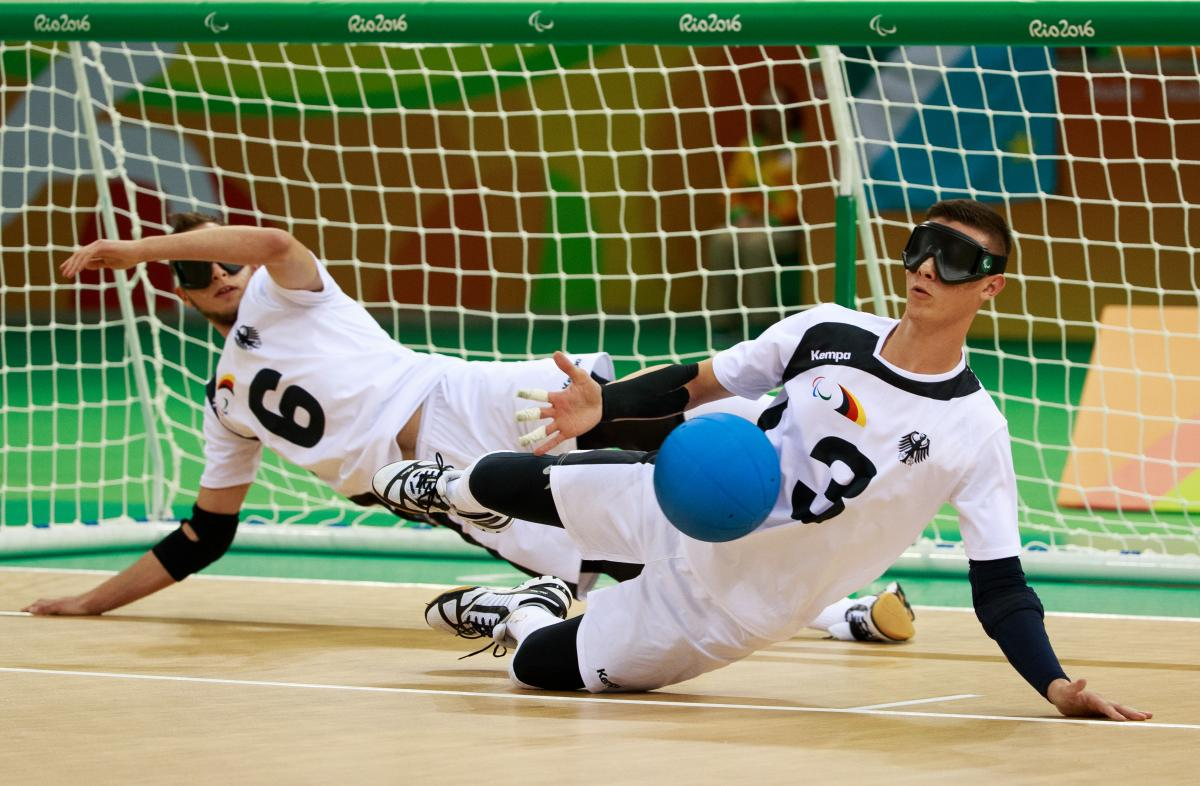
\includegraphics[width=0.8\textwidth]{Images/goalball.JPG}
\caption{Goalball}
\label{fig:my_image}
\end{figure}

\item Categories and Classifications
    \begin{itemize}
    \item All players in goalball are classified as B1, B2, or B3, based on the severity of their visual impairment. B1 players have the least visual acuity, while B3 players have the most. 
    \item All players wear eyeshades to ensure a level playing field, regardless of their classification. 
    \item This system fosters fair competition and highlights the impressive skills and strategies employed by athletes with visual impairments in this unique sport.
    \end{itemize}

\end{enumerate}